\chapter{Results}
The three path planners (NHV, N-NHV, and MCPP) introduced in Chapter \ref{ch:pp} all aim to reduce the overall prediction uncertainty of a field given a limited amount of flight time. They accomplish the task by calculating variances of a target field's predictions and attempting to choose a trajectory that reduces overall uncertainty. 

\section{Comparing The Method}
A common approach to exploration and patrolling problems is the use of a spiral, zig-zag, or lawn mower pattern. The methods introduced will be compared to equally time limited version of a zig-zagging approaches seen in Nikhil Nigam, et al. Control and Design of Multiple Unmanned Air Vehicles for a Persistent Surveillance Task (Part II.C.3, Figure 6, \cite{nigam:zigzag}). The method, for the sake of fairer comparison, will run a Kriging prediction and variance calculation on the samples taken using the zig-zag explorer. This is to generate measurable and comparable metrics against the path planners introduced. The path planners introduced will be compared against the zig-zag exploration method shown in Figure \ref{fig:zigzag4}.

\begin{figure}[hbt!]
	\centering
	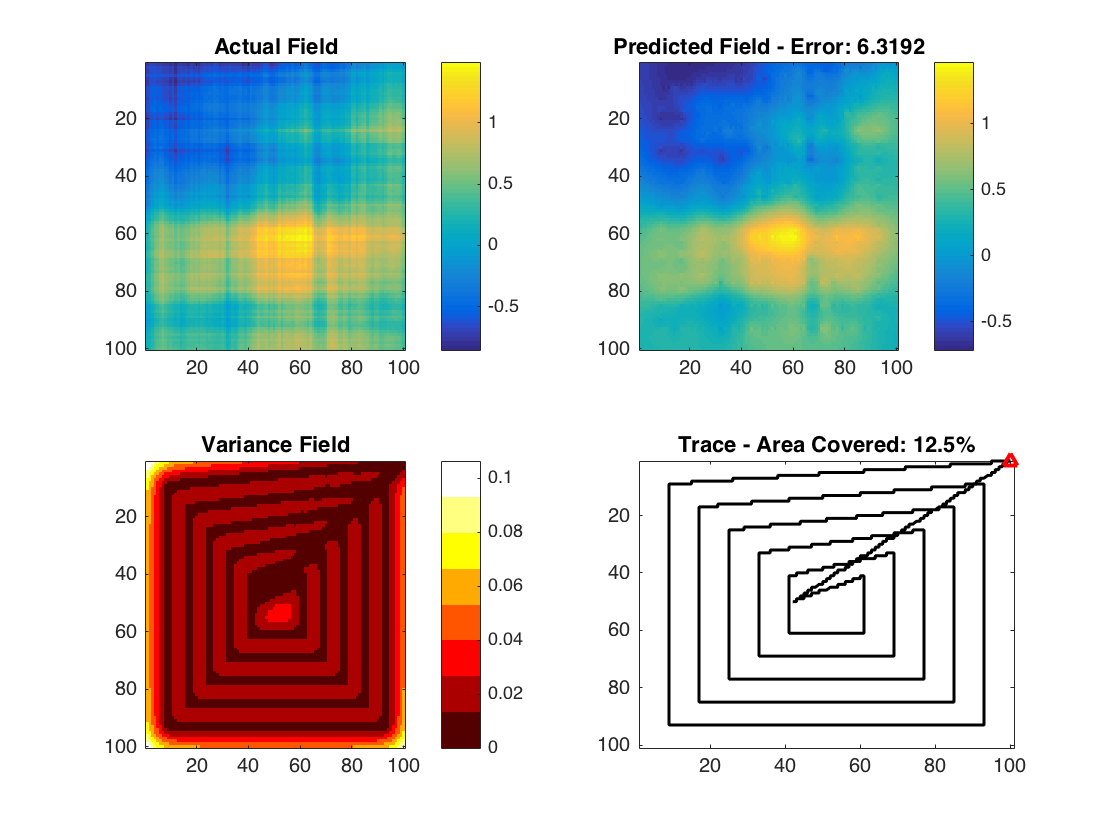
\includegraphics[width=0.9\linewidth]{figures/zigzag_4panel.png}
	\captionsetup{skip=0.20\baselineskip,size=footnotesize}
	\caption{Zig-Zag exploration method with a line spacing of $r = 8$ units. A Kriging prediction and variance calculation is computed after completing the maneuver. The actual field that is being explored is shown in the upper left. The current prediction of the actual field is shown in the upper right. The variance of the current prediction of the field is shown in the lower left. The trace of the exploration vehicle's path taken to the point of termination (in red) is shown in the lower right panel. All distance units are in meters.}
	\label{fig:zigzag4}
\end{figure}

\subsection{Prediction Error Calculation}
The quality of each path planner will be judged by its ability to explore a field in a fixed amount of time. The prediction error of each method will be used as a metric of path planning quality. The actual values of the fields scanned are known in simulation, and for each rerouting iteration, the predictions and prediction errors will be recalculated.

The prediction error value for each field prediction made will be the mean of every vesicles root mean square (RMS) error (element by element).

\subsection{Variance Drop Calculation}
The variance of every target field over each iteration will be the average prediction variance of the field after every prediction recalculation. This criteria is introduced in Section \ref{sec:fielduncert} on field uncertainty. This metric relates prediction quality of the path planner to its predicted prediction quality. A drop in variance over iterations should signal a better prediction of the target field over that iteration, and less overall uncertainty of the target field.

\subsection{Varying Target Field Sizes}
The effectiveness of the method introduced varies based on the area of the target field being explored. For small fields, a naive zig-zag exploration may be more efficient and less computationally expensive. By modulating the dimensions of the target field, a comparison can be drawn demonstrating the effectiveness of the method versus a naive zig-zag approach.

The exploration techniques introduced will be compared against the zig-zag technique for a variety of area coverage limits. The spacing of the zig-zag traces will are set to

\begin{equation}
	r = \frac{A_{scan}}{2}
\end{equation}

Where $A_{scan}$ is the maximum area to scan. For a maximum fraction of the field to scan, $c_max$, $A_{scan} = wc_{max}$.

\subsubsection{$20 \times 20$ Target Field Size}
The methods introduced will be compared to one another and the zig-zag method in terms of variance drop and prediction error on a set of $5$ randomly generated geospatially autocorrelated fields with $20\times20$ vesicles.

\begin{table}[ht!]
\centering
	\begin{tabular}{ |p{3cm}||p{1cm}|p{1cm}|p{1cm}|p{1cm}|p{1cm}|  }
		\hline
		\multicolumn{6}{|c|}{$20 \times 20$ Size Final Field Prediction Error} \\
		\hline
		Coverage Limit & 20\% & 30\% & 40\% & 50\% & 75\% \\
		\hline
		Zig-Zag        & .. & .. & .. & 2.3060 & .. \\
		NHV            & .. & .. & .. & 2.1858 & .. \\
		N-NHV          & .. & .. & .. & 2.1765 & .. \\
		MCPP           & .. & .. & .. & 2.1888 & .. \\
		\hline
	\end{tabular}
	\caption{Comparing field prediction errors for varying coverage limitations on a $20 \times 20$ size field.}
    \label{tab:20fieldprederr}
\end{table}

\begin{figure}[hb!]
	\centering
	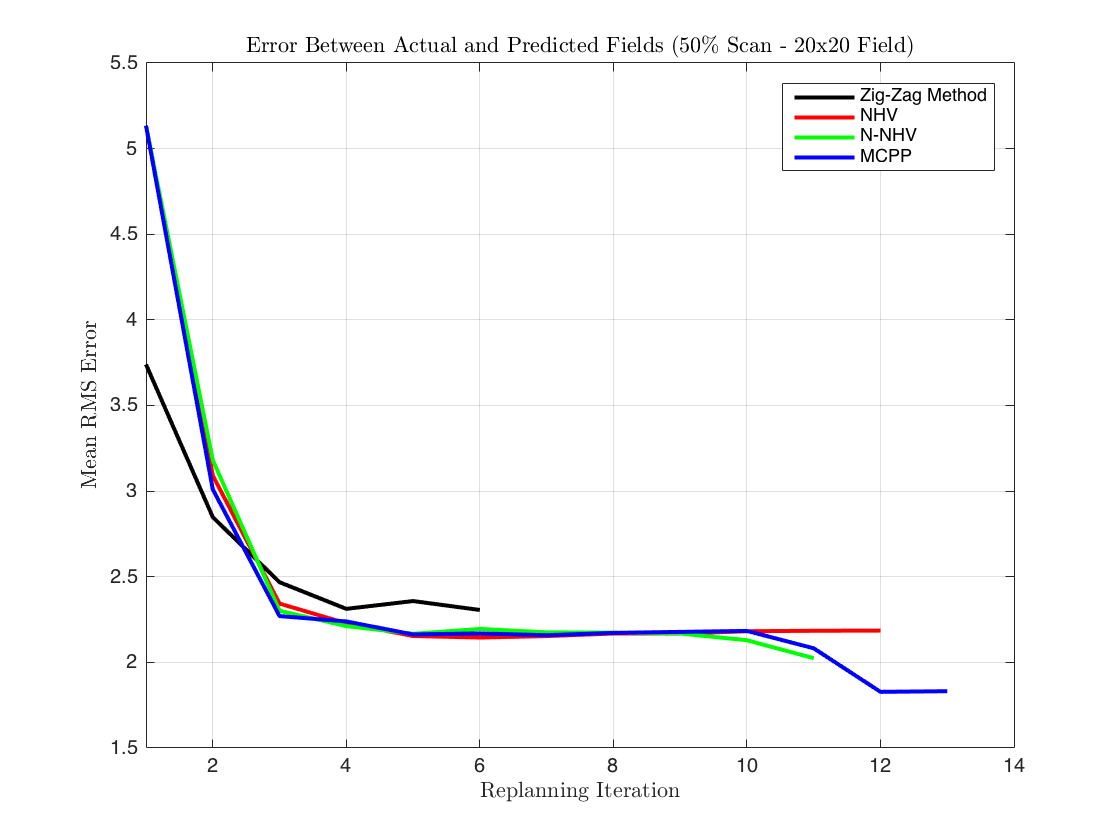
\includegraphics[width=0.8\linewidth]{figures/pred_error_20x20_50percent_5runs.png}
    \captionsetup{skip=0.20\baselineskip,size=footnotesize}
	\caption{Normalized prediction error drops per replanning iteration averaged over exploring 5 randomly generated target fields of size $20 \times 20$ at a $50\%$ scan. The predictions for the zig-zag method are recalculated at every turn.}
\end{figure}

\begin{table}[ht!]
\centering
	\begin{tabular}{ |p{3cm}||p{1cm}|p{1cm}|p{1cm}|p{1cm}|p{1cm}|  }
		\hline
		\multicolumn{6}{|c|}{$20 \times 20$ Size Final Field Prediction Variance} \\
		\hline
		Coverage Limit & 20\% & 30\% & 40\% & 50\% & 75\% \\
		\hline
		Zig-Zag        & .. & .. & .. & 1.5046 & .. \\
		NHV            & .. & .. & .. & 0.3822 & .. \\
		N-NHV          & .. & .. & .. & 0.3819 & .. \\
		MCPP           & .. & .. & .. & 0.3238 & .. \\
		\hline
	\end{tabular}
	\caption{Comparing field prediction errors for varying coverage limitations on a $20 \times 20$ size field.}
    \label{tab:20fieldvar}
\end{table}

\begin{figure}[hb!]
	\centering
	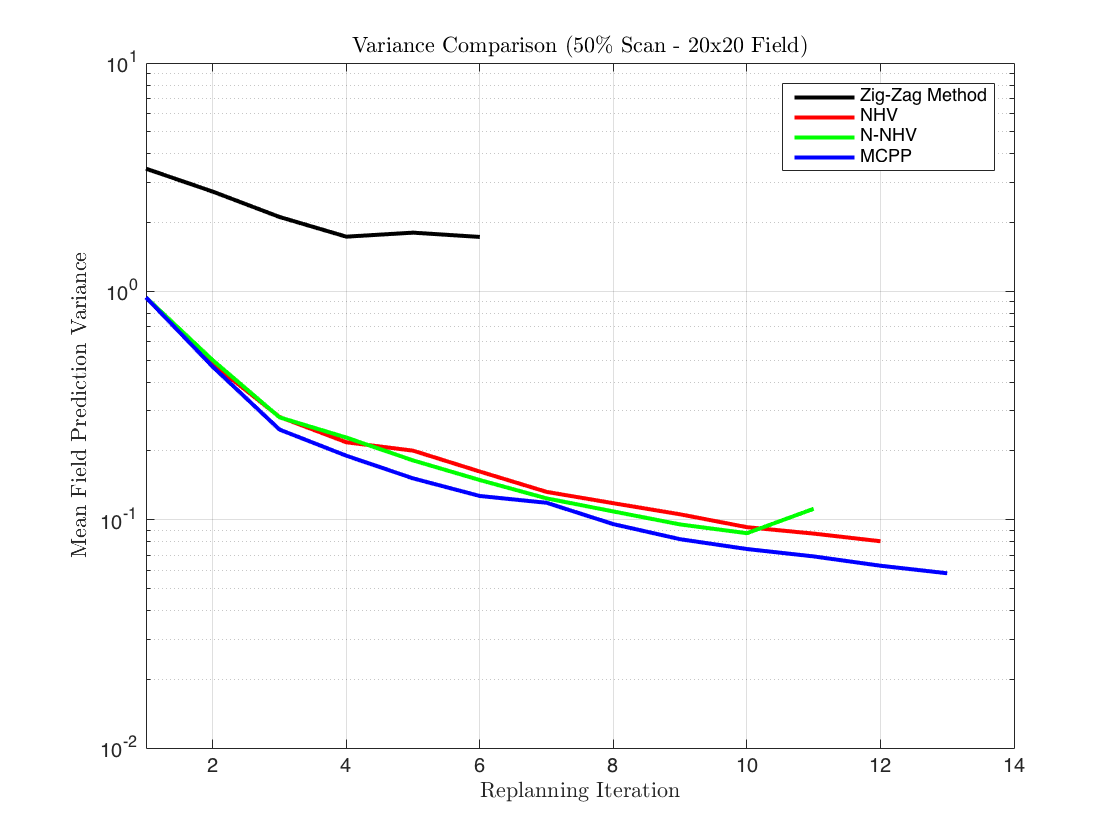
\includegraphics[width=0.8\linewidth]{figures/vars_semilogy_20x20_50percent_5runs.png}
    \captionsetup{skip=0.20\baselineskip,size=footnotesize}
	\caption{Logarithmic variance drops per replanning iteration averaged over exploring 5 randomly generated target fields of size $20 \times 20$ at a $50\%$ scan. The variance for the zig-zag method are recalculated at every turn.}
\end{figure}

\subsubsection{$50 \times 50$ Target Field Size}
The methods introduced will be compared to one another and the zig-zag method in terms of variance drop and prediction error on a set of $5$ randomly generated geospatially autocorrelated fields with $50\times 50$ vesicles.

\begin{table}[htb!]
\centering
	\begin{tabular}{ |p{3cm}||p{1cm}|p{1cm}|p{1cm}|p{1cm}|p{1cm}|  }
		\hline
		\multicolumn{6}{|c|}{$50 \times 50$ Size Final Field Prediction Error} \\
		\hline
		Coverage Limit & 1\% & 5\% & 10\% & 20\% & 50\% \\
		\hline
		Zig-Zag        & .. & .. & .. & .. & .. \\
		NHV            & .. & .. & .. & .. & .. \\
		N-NHV          & .. & .. & .. & .. & .. \\
		MCPP           & .. & .. & .. & .. & .. \\
		\hline
	\end{tabular}
	\caption{Comparing field prediction errors for varying coverage limitations on a $50 \times 50$ size field.}
    \label{tab:50fieldprederr}
\end{table}

\begin{table}[htb!]
\centering
	\begin{tabular}{ |p{3cm}||p{1cm}|p{1cm}|p{1cm}|p{1cm}|p{1cm}|  }
		\hline
		\multicolumn{6}{|c|}{$50 \times 50$ Size Final Field Prediction Variance} \\
		\hline
		Coverage Limit & 10\% & 20\% & 25\% & 50\% & 75\% \\
		\hline
		Zig-Zag        & .. & .. & .. & .. & .. \\
		NHV            & .. & .. & .. & .. & .. \\
		N-NHV          & .. & .. & .. & .. & .. \\
		MCPP           & .. & .. & .. & .. & .. \\
		\hline
	\end{tabular}
	\caption{Comparing field prediction errors for varying coverage limitations on a $50 \times 50$ size field.}
    \label{tab:50fieldvar}
\end{table}

\section{Result Conclusions}
write this part.